\section{Refinement-based game semantics}

This section introduces the category $\mathcal{G}$ of games and strategies
we use to interpret the behavior of low-level interacting components.
$\mathcal{G}$ has no high-order structure,
which simplifies the definition of games considerably.
On the other hand,
our definition of strategy is generalized to accomodate specifications,
and the morphisms of $\mathcal{G}$ are equipped with a notion of refinement
suitable for our purposes.

\subsection{Behaviors and specifications} %{{{

\subsubsection{Non-determinism} %{{{

We will use non-determinism
to express specifications allowing a range of behaviors.
Accordingly,
our semantic domain will be equipped with a lattice structure
interpreted in the following way.

Given $x, y : \mathcal{B}(A)$,
their supremum $x \vee y : \mathcal{B}(A)$
is the smallest specification that permits the behavior of either;
on the other hand $x \wedge y : \mathcal{B}(A)$ can be interpreted as
the largest specification requiring that $x$ and $y$ both be satisfied.
The least element $\bot$
is a specification that can never be satisfied;
the greatest element $\top$
is the specification that is always satisfied.

%}}}

\subsubsection{Undefined behaviors} %{{{

Low-level language semantics and specifications
often contain \emph{undefined behaviors}:
there are circumstances under which the behavior of the system
is entierly unrestricted;
any execution that reaches such circumstances is said to ``go wrong''.
A computation that goes wrong can be refined
from that point on by any other computation.

We model undefined behavior using the distinguished outcome $\lightning$,
which represents a computation whose behavior is undefined
from that point on.
Accordingly,
the greatest element $\top$ of our semantic lattice
will be the computation that immediately goes wrong.

%}}}

\subsubsection{Silent divergence} %{{{

Finally,
[explain that divergence is incomparable with
other behaviors rather than $\top$ or $\bot$].

%}}}

In the following section,
we explain how these aspects of our model
are captured in our definition of the \emph{interaction} monad,
which serves as the basis for
our definition of strategies.

%}}}

\subsection{The interaction monad} %{{{

The usual definition of strategies as
prefix-closed sets of traces
offers many advantages:
it is relatively simple;
the ordering properties of powerset lattices
are straightforward and well-understood;
and as a trace semantics
it is particularly well-suited to obtain
full abstraction results
with respect to a system's externally observable behavior.

More operational approaches,
like the transition systems used to define
the semantics of CompCert languages,
[means we have to deal with branching and
use complex equivalence relations,
but on the other hand
are closer to the system's concrete behavior
and allow intuitive operational reasoning.]

Before we introduce games and strategies
in the following sections,
we define the \emph{interaction} monad $\mathcal{I}_{M,N}$.
Using a monad as the base of our model
introduces a notion of sequential composition
which makes it possible to define strategies
in a compositional and operational way.

\subsubsection{Overview} %{{{

The \emph{interaction monad} models
a computation which may interact with its environment.
The computation can perform and output $m \in M$,
at which point it will be suspended
until an input $n \in N$ is received from the environment.
This is modelled by the operation:
\[
    \kw{interact} : M \rightarrow \mathcal{I}_{M,N}(N) \,.
\]

Additionally,
to model specifications which permit a range of possible behaviors,
we allow non-deterministic strategies.
The interaction monad is equipped with a complete refinement lattice,
which we extend with a distinguished greatest element:
\[
    \top : I_{M,N}(A) \,,
\]
representing a computation whose behavior is undefined.

Finally,
we model non-deterministic iteration with the operator:
\[
     -^\infty : (A \rightarrow \mathcal{I}_{M,N}(A)) \rightarrow
                (A \rightarrow \mathcal{I}_{M,N}(A)) \,.
\]
Notably,
$-^\infty$ is different from
the Kleene star associated with the refinement lattice
because we account for silent divergence as a specific behavior,
incomparable with terminating computations,
rather than identifying it with
the unsatisfiable specification $\bot$
or the undefined behavior $\top$.

Using the interaction monad,
alternating strategies for a game with
opponent moves in $M^\kw{O}$ and
proponent moves in $M^\kw{P}$,
where $\kw{O}$ is expected to make the first move,
can be modelled as computations of type:
\[
    M^\kw{O} \rightarrow
      \mathcal{I}_{M^\kw{P}, M^\kw{O}}(\varnothing) \,.
\]

%}}}

\subsubsection{Definition} %{{{

Following the usual approach,
we formalize strategies as prefix-closed sets of plays.
We do not allow strategies to restrict the move available to $\kw{O}$,
so the plays we will consider are odd-length sequences of moves.
To support the monadic structure and account
for silent divergence and undefined behaviors,
we extend them with the
terminal moves $v \in X$, $\Delta$, and $\lightning$:
\[
    \mathcal{T}_{M,N}(X) :=
      (M N)^* \times (M + X + \{\Delta, \lightning\})
\]
Any trace is considered a prefix of $(\varepsilon, \lightning)$,
so that our extended prefix relation on $\mathcal{T}_{M,N}(X)$
is defined by the rules:
\[
  \begin{array}{r@{\:\sqsubseteq\:}l}
    (\varepsilon, m) & (mn, s) \\
    (\varepsilon, v) & (\varepsilon, v) \\
    (\varepsilon, \Delta) & (\varepsilon, \Delta) \\
    (\varepsilon, \lightning) & (s, p)
  \end{array}
  \quad
  \AxiomC{$(s, p) \sqsubseteq (t, q)$}
  \UnaryInfC{$(mns, p) \sqsubseteq (mnt, q)$}
  \DisplayProof
\]
An interactive computation is
a prefix-closed set of traces:
\[
    \mathcal{I}_{M,N}(X) :=
    \{ T \subseteq \mathcal{T}_{M,N}(X) \mid
       {\sqsubseteq}^{-1}(T) \subseteq T \}
\]

Note that since any trace is a prefix of $\lightning$,
a computation which admits a trace ending with $\lightning$
will also admit all possible interactions
sharing the same initial segment. 
This allows us to define our notion of refinement
as simple trace containment.
For $x, y \in \mathcal{I}_{M,N}(X)$, refinement is defined as:
\[
    x \sqsubseteq y \Leftrightarrow x \subseteq y
\]
Since unions and intersections
preserve prefix closure,
they induce a lattice structure on $\mathcal{I}_{M,N}(X)$.

%}}}

\subsubsection{Monad operations} %{{{

The monad's unit associates to each value $v \in X$
the computation with a single trace $(\varepsilon, v)$:
\[
    \kw{ret}_X(v) := \{ (\varepsilon, v) \} \,.
\]
The binding operation corresponds to
the sequential composition of
a computation $x \in \mathcal{I}_{M,N}(A)$ and
a continuation $f : A \rightarrow \mathcal{I}_{M,N}(B)$.
The result is a computation in $\mathcal{I}_{M,N}(B)$ which
contains the traces of $x$ where
any final value $v$ has been replaced with
all possible traces in $f(v)$:
\begin{align*}
    s \bind f := &\:\{ (s, \: r) \mid (s, r) \in x \wedge r \notin A \} \\
      \cup &\:\{ (st, r) \mid (s, a) \in x \wedge (t, r) \in f(a) \}
\end{align*}
It is straightforward to verify that
the monad laws hold:
\begin{align*}
  \kw{ret}(v) \bind f &= f(v) \\
  x \bind \kw{ret} &= x \\
  x \bind (v \mapsto f(v) \bind g) &= (x \bind f) \bind g
\end{align*}

%}}}

\subsubsection{Interaction} %{{{

The interaction primitive
$\kw{interact} : M \rightarrow \mathcal{I}_{M,N}(N)$
can be defined as follows:
\[
    \kw{interact}(m) := \{ (\varepsilon, m), (mn, n) \mid n \in N \}
\]
That is,
$\kw{interact}(m)$ first emits the output $m$,
then returns the input $n$ received from the environment.

Conversely,
the following operator
will allow us to evaluate a computation
while ``monitoring'' its interactions:
\[
    \kw{next} :
       \mathcal{I}_{M,N}(X) \rightarrow
       \mathcal{I}_{P,Q}(X + M \times (N \rightarrow \mathcal{I}_{M,N}(X)))
\]
When the computation $x$ silently terminates, diverges, or goes wrong,
then $\kw{next}(x)$ will exhibit the same behavior:
\begin{align*}
    \kw{next}(\kw{ret}(a)) &= \kw{ret}(i_1(a)) \\
    \kw{next}(\Omega) &= \Omega \\
    \kw{next}(\top) &= \top
\end{align*}
However,
if $x$ attempts to interact,
then $\kw{next}(x)$ will suspend it,
and return the output $m \in M$ attempted by $x$,
as well as a continuation $N \rightarrow \mathcal{I}_{M,N}(X)$
which can be used to resume the computation
on an input $n \in N$.
In particular,
\[
    \kw{next}(\kw{interact}(m)) = \kw{ret}(i_2(m), \kw{ret}) \,.
\]
The operator can be defined as follows:
\begin{align*}
    \kw{next}(x) &= \{ (\varepsilon, i_1(v)) \mid
                       (\varepsilon, v) \in x \wedge
                       v \in X \} \\
              &\cup \{ (\varepsilon, r) \mid
                       (\varepsilon, r) \in x \wedge
                       r \in \{\Delta,\lightning\} \} \\
              &\cup \{ (\varepsilon, i_2(m, \delta_m(x))) \mid
                       (\varepsilon, m) \in x \wedge
                       m \in M \} \,,
\end{align*}
where the derivative
$\delta(x) :
   \mathcal{I}_{M,N}(X) \rightarrow M \rightarrow N \rightarrow
   \mathcal{I}_{M,N}(X)$
is defined as:
\[
    \delta(x)(m)(n) := \{ (s, r) \mid (mns, r) \in x \} \,.
\]

%}}}

\subsubsection{Iteration} %{{{

A Kleisli morphism $f : A \rightarrow \mathcal{I}_{M,N}(A)$
can be iterated as follows.
First,
we identify silently diverging computations by defining:
\[
    f_\Delta(v) :=
      f \cup \{ \Delta \mid \forall n, \exists x \notin M, f^n(v) \ni x \}
\]
Then the iteration of $f$ is:
\[
    f^\infty(v) :=
      \bigvee_{n} f_\Delta^n \,.
\]
Here $f^n$ refers to the $n$-fold composition of $f$,
where:
\begin{align*}
    f^0(a) &:= \kw{ret}(a) \\
    f^{n+1}(a) &:= f^n(a) \bind f \,.
\end{align*}

%}}}

\subsubsection{Relations} %{{{

The powerset monad $\mathcal{P}$
can be embedded into the monad $\mathcal{I}_{M,N}$
using the natural transformation
$\eta^\mathcal{P}_X : \mathcal{P}(X) \rightarrow \mathcal{I}_{M,N}(X)$
defined as:
\[
    \eta^\mathcal{P}_X(V) := \{ (\varepsilon, v) \mid v \in V \}
\]
In particular,
a relation $R : A \rightarrow \mathcal{P}(B)$
can be interpreted as the Kleisli morphism
$\eta^\mathcal{P}_B \circ R : A \rightarrow \mathcal{I}_{M,N}(B)$.

\begin{example} \label{ex:ts}
Consider a transition system $\alpha = (S, I, {\rightarrow}, F)$,
where
$S$ is a set of states,
$I : \mathcal{P}(S)$
is a set of initial states,
${\rightarrow} : S \rightarrow \mathcal{P}(S)$
is a transition relation, and
$F : S \rightarrow \mathcal{P}(A)$
associate potential output values to each state.
The behavior of $\alpha$ can be expressed as:
\[
    \llbracket \alpha \rrbracket :=
    \eta^\mathcal{P}_S(I) \bind
    (\eta^\mathcal{P}_S \circ {\rightarrow})^\infty \bind
    (\eta^\mathcal{P}_S \circ F)
    : \mathcal{I}_{M,N}(A) \,.
\]
\end{example}

We will use this pattern extensively
when defining constructions on strategies
which may introduce silent divergence.

%}}}

%}}}

\subsection{Abstraction} %{{{

We now consider the problem of relating the interactive computations
$x_1 \mathcal{I}_{M_1,N_1}(X_1)$ and
$x_2 \mathcal{I}_{M_2,N_2}(X_2)$
whose inputs, outputs, and results are taken in different sets.
We will use Kripke logical relations to relate these components,
so that the correspondance between the two interactions
can be sensitive to the history of the computation.

\begin{definition}
For sets of inputs $M_1, M_2$, outputs $N_1, N_2$, and results $X_1, X_2$,
a \emph{simulation convention} between them
is a tuple $\mathbb{R} = \langle W, \leadsto, R_M, R_N, R_X \rangle$
where $\langle W, \leadsto \rangle$ is a Kripke frame, and
$R_M : \mathcal{R}_W(M_1, M_2)$,
$R_N : \mathcal{R}_W(N_1, N_2)$,
$R_X : \mathcal{R}_W(X_1, X_2)$
are $W$-indexed Kripke logical relations
between the respective sets of inputs, outputs and results.

The identity simulation convention is defined as
$\mathbbm{1} := \langle \{*\}, \{(*,*)\}, {=}, {=}, {=} \rangle$.
The composition of
the simulation conventions $\mathbb{R}$ and $\mathbb{S}$ is:
\[
    \mathbb{R} \cdot \mathbb{S} :=
      \langle
        W_\mathbb{R} \times W_\mathbb{S}, \:
        {\leadsto}_\mathbb{R} \times {\leadsto}_\mathbb{S}, \:
        R_M \cdot S_M, \:
        R_N \cdot S_N, \:
        R_X \cdot S_X
      \rangle \,,
\]
where $R \cdot S$ denotes the Kripke relation defined by:
\[
    (w_1, w_2) \Vdash R \cdot S \: := \:
      (w_1 \Vdash R) \cdot (w_2 \Vdash S) \,.
\]

\end{definition}

Simulation conventions relate interactions which have the same ``shape'',
in the sense that there is a one-to-one correspondance between
the inputs and outputs of $x_1$ and $x_2$.
Nevertheless,
extending a simulation convention $\mathbb{R}$ to computations
is complicated by the alternating roles of the system and the environment.
Our goal will be to define a Kripke relator:
\[ {\le}_\mathbb{R} \: = \:
   \mathcal{I}^\le_{R_M,R_N}(R_X) \: : \:
   \mathcal{R}_W(\mathcal{I}_{M_1,N_1}(X_1), \mathcal{I}_{M_2,N_2}(X_2)) \]
such that $x_1 \le_\mathbb{R} x_2$
whenever $x_1$ is simulated by $x_2$ according to the convention $\mathbb{R}$.
We will proceed by defining a mapping:
\[ \mathbb{R}^*_w : \mathcal{I}_{M_2,N_2}(X_2) \rightarrow
                    \mathcal{I}_{M_1,N_1}(X_1) \, \]
such that $\mathbb{R}^*_w(x_2)$ is
the largest computation in $\mathcal{I}_{M_1,N_1}(X_1)$
simulated by $x_2$.
Accordingly,
we will define:
\[ w \Vdash x_1 \le_\mathbb{R} x_2 \: \Leftrightarrow \:
   x_1 \sqsubseteq \mathbb{R}^*_w(x_2) \,. \]

In the presence of different levels of abstraction
related by a convention $\mathbb{R}$,
the mapping $\mathbb{R}^*$ will allow us to embed a high-level specification
into a low-level semantic domain
where it can be compared with
the concrete behavior of the system we wish to verify.
On the other hand, $\le_\mathbb{R}$
allows us to express abstraction relationally,
and in particular the corresponding properties of
the primitives of the interaction monad
will help us construct
simulations between
structurally similar computations
at different levels of abstraction.

\subsubsection{Embedding}

The mapping $\mathbb{R}^*$ is defined as follows.

\begin{definition}
For a simulation convention $\mathbb{R} = \langle R_M, R_N, R_X \rangle$
and a computation $x_2 : \mathcal{I}_{M_2, N_2}(X_2)$,
the computation $\mathbb{R}^*_w(x_2)$ is defined by the rules:
\begin{gather*}
  \AxiomC{$(\varepsilon, v_2) \in x_2$}
  \AxiomC{$v_1 \ifr{w \Vdash R_X} v_2$}
  \BinaryInfC{$(\varepsilon, v_1) \in \mathbb{R}^*_w(x_2)$}
  \DisplayProof
  \qquad
  \AxiomC{$(\varepsilon, \Delta) \in x_2$}
  \UnaryInfC{$(\varepsilon, \Delta) \in \mathbb{R}^*_w(x_2)$}
  \DisplayProof
  \qquad
  \AxiomC{$(\varepsilon, \lightning) \in x_2$}
  \UnaryInfC{$t \in \mathbb{R}^*_w(x_2)$}
  \DisplayProof
  \\[1ex]
  \AxiomC{$(\varepsilon, m_2) \in x_2$}
  \AxiomC{$w \leadsto w'$}
  \AxiomC{$m_1 \ifr{w' \Vdash R_M} m_2$}
  \TrinaryInfC{$(\varepsilon, m_1) \in \mathbb{R}^*_w(x_2)$}
  \DisplayProof
  \\[1ex]
  \AxiomC{$
    \begin{array}{c}
      (\varepsilon, m_2) \in x_2 \qquad
      w \leadsto w' \qquad
      m_1 \ifr{w' \Vdash R_M} m_2
      \\[.3ex]
      \forall \: w'' \, n_2 \:.\:
        w' \leadsto w'' \: \wedge \:
        n_1 \ifr{w'' \Vdash R_N} n_2 \: \Rightarrow \:
        t_1 \in \mathbb{R}^*_{w''}(\delta(x_2, m_2)(n_2))
    \end{array}$}
  \UnaryInfC{$m_1 n_1 t_1 \in \mathbb{R}^*_w(x_2)$}
  \DisplayProof
\end{gather*}
\end{definition}

Note that $\mathbbm{1}^*_w(x) = x$
and that $(\mathbb{R} \cdot \mathbb{S})^* = \mathbb{S}^* \circ \mathbb{R}^*$.
In addition,
$\mathbb{R}^*$ can be extended to Kleisli morphisms as follows:
\[
    \mathbb{R}^*_w(f) :=
       a_1 \mapsto \bigwedge_{
         \begin{array}{c}
           w \leadsto w' \\
           a_1 \ifr{w' \Vdash R_A} a_2
         \end{array}}
         \mathbb{R}^*_{w'}(f(a_2))
\]

\subsubsection{Relator}

We now seek to use the embedding defined in the previous section
to generalize the refinement relation
to allow relational reasoning between interactive computations
which may use different types of outputs, inputs and values.

\begin{definition}
For a simulation convention $\mathbb{R} = \langle R_M, R_N, R_X \rangle$,
a world $w$,
and two computations
$x_1 : \mathcal{I}_{M_1, N_1}(X_1)$ and
$x_2 : \mathcal{I}_{M_2, N_2}(X_2)$,
we say that
\emph{$x_1$ is simulated at $w$ by $x_2$ according to $\mathbb{R}$}
and write:
\[
    x_1 \ifr{w \Vdash {\le}_\mathbb{R}} x_2
    \quad \mbox{or} \quad
    x_1 \ifr{w \Vdash \mathcal{I}^\le_{R_M,R_N}(R_X)} x_2
\]
whenever $x_1 \sqsubseteq \mathbb{R}^*_w(x_2)$.
\end{definition}

Kleisli morphisms can be compared
by the relation $\Box(R_A \rightarrow \mathcal{I}^\le_{R_M,R_N}(R_B))$.
Identity and composition yield
${\le}_\mathbbm{1} = {\sqsubseteq}$ and
${\le}_{\mathbb{R} \cdot \mathbb{S}} =
 {\le}_\mathbb{R} \cdot {\le}_\mathbb{S}$.
More generally,
the following properties make
$\mathcal{I}_{M,N}^\le$ into a \emph{relator} \cite{something}:
\begin{align*}
  {=}_{\mathcal{I}_{M,N}(X)} &\subseteq \mathcal{I}_{M,N}^\le(=_X) \\
  \mathcal{I}_{M,N}^\le(R) \cdot \mathcal{I}_{M,N}^\le(S) &\subseteq
    \mathcal{I}_{M,N}^\le(R \cdot S) \\
  R \subseteq S \Rightarrow
    \mathcal{I}_{M,N}^\le(R) &\subseteq \mathcal{I}_{M,N}^\le(S) \,.
\end{align*}
Note that $\mathcal{I}_{M,N}(=)$ corresponds to $\sqsubseteq$,
so that in particular, $\mathcal{I}_{M,N}^\le(R)$ is compatible with $\sqsubseteq$
in the following sense:
\begin{align*}
    {\sqsubseteq} \cdot \mathcal{I}_{M,N}^\le(R) &\:\subseteq\:
      \mathcal{I}_{M,N}^\le(R) \\
    \mathcal{I}_{M,N}^\le(R) \cdot {\sqsubseteq} &\:\subseteq\:
      \mathcal{I}_{M,N}^\le(R)
\end{align*}

The relator is also compatible with the monad operations
in the sense that the following relational properties hold:
\begin{align*}
  \kw{ret} &:
    {}\Vdash R_X \rightarrow \mathcal{I}^\le_{R_M,R_N}(R_X) \\
  \bind &:
    (\Vdash R_X \rightarrow
     \mathcal{I}^\le_{R_M,R_N}(R_Y)) \rightarrow
    (\Vdash \mathcal{I}^\le_{R_M,R_N}(R_X) \rightarrow
     \mathcal{I}^\le_{R_M,R_N}(R_Y)) \\
  \kw{interact} &:
    (\Vdash (\Diamond R_M) \rightarrow
     \mathcal{I}^\le_{R_M,R_N}(R_N)) \\
  \kw{next} &:
    (\Vdash \mathcal{I}^\le_{R_M,R_N}(R_X) \rightarrow
     R_X +
     \Diamond (R_M \times
     \Box (R_N \rightarrow \mathcal{I}^\le_{R_M,R_N}(R_X)))) \\
  -^\infty &:
    (\Vdash R_X \rightarrow \mathcal{I}^\le_{R_M,R_N}(R_X)) \rightarrow
    (\Vdash R_X \rightarrow \mathcal{I}^\le_{R_M,R_N}(R_X)) \\
  \eta^\mathcal{P} &:
    (\Vdash \mathcal{P}^\le(R_X) \rightarrow
     \mathcal{I}^\le_{R_M,R_N}(R_X))
\end{align*}
Together,
these properties allow us to construct
heterogenous simulations
between monadic terms with similar structures.

\begin{example} \label{ex:sim}
Building on our previous example,
consider
$\alpha_1 = (S_1, I_1, {\rightarrow}_1, F_1)$ and
$\alpha_2 = (S_2, I_2, {\rightarrow}_2, F_2)$
two transition systems,
together with a relation
$R : \mathcal{R}(S_1, S_2)$
satisfying:
\begin{gather*}
  I_1 \ifr{\mathcal{P}^\le(R)} I_2 \\
  {\rightarrow}_1 \ifr{R \rightarrow \mathcal{P}^\le(R)} {\rightarrow}_2 \\
  F_1 \ifr{R \rightarrow \mathcal{P}^\le(=)} F_2
\end{gather*}
That is, $R$ is a simulation relation between $\alpha_1$ and $\alpha_2$.
Then by using the properties above
following the structure of $\llbracket - \rrbracket$,
we can show that:
\[
    \llbracket \alpha_1 \rrbracket \sqsubseteq
    \llbracket \alpha_2 \rrbracket \,.
\]
\end{example}

%}}}


%
%\subsection{Behavior specifications}
%
%\subsubsection{Simulations}
%
%The pointwise extension of the relator $\mathcal{B}^\sqsubseteq$
%to the interaction monad
%yields a notion of simulation for interactive computations.
%However,
%it is limited to computations which have identical interactions
%with their environment,
%and for which the way values are related
%is independent of the histories of the computations.
%In the following
%we present a ternary Kripke relator $\mathcal{I}^+_{\preceq_M,\preceq_N}(R)$
%which allows us to compare interactions
%operating with different inputs and outputs,
%and for whose outcomes may be related in a way
%sensitive to the interactions' histories.
%
%Suppose we have a set of worlds $W$
%together with two labelled Kripke frames
%${\leadsto}^\kw{O} : M_1^O \times M_2^O \rightarrow \mathcal{R}(W, W)$ and
%${\leadsto}^\kw{P} : M_1^P \times M_2^P \rightarrow \mathcal{R}(W, W)$.
%These can be used to define a form of rely-guarantee simulation
%between two interactive computations
%$x_1 : \mathcal{I}_{M_1^\kw{P},M_1^\kw{P}}(A_1)$ and
%$x_2 : \mathcal{I}_{M_2^\kw{P},M_2^\kw{P}}(A_2)$
%in the following way.
%The computations will be related at $w$
%if for all interactions $s = (m_1, n_1) \cdot (m_2, n_2) \cdots (m_k, n_k)$
%the following holds:
%\[
%    x_1(s)
%    \ifr{w \Vdash
%         \langle m_1 \rangle [n_1] \cdots
%         \langle m_k \rangle [n_k] \,
%         \mathcal{B}(\Diamond + R)}
%    x_2(s) \,,
%\]
%where $\Diamond : \mathcal{R}_W(M_1^\kw{P}, M_2^\kw{P})$
%is the relation defined as:
%\[
%    m_1 \ifr{w \Vdash \Diamond} m_2 \Leftrightarrow
%      \exists w' \,.\, w \stackrel{m_1,m_2}{\leadsto^\kw{P}} w'
%\]
%
%[Define substitution?]
%


\subsection{Games and strategies} %{{{

\subsubsection{Elementary games} %{{{

The elementary games which underlie
our category of games and strategies
can be decribed in the following way.

\begin{definition} % elementary game {{{
An \emph{elementary game} is a pair
$A = \langle M_A^\kw{Q}, M_A^\kw{A} \rangle$, where
$M_A^\kw{Q}$ is a set of \emph{questions}, and
$M_A^\kw{A}$ is a set of \emph{answers}.
\end{definition}
%}}}

The game proceeds as follows:
first $\kw{O}$ chooses a question,
then $\kw{P}$ chooses an answer.
On their own,
elementary games present little interest.
Instead, we will focus on
the composite games $A \rightarrow B$
described in the following section.

%
%Elementary games place no restrictions
%on the valid plays,
%but this can be specified relationally.
%
%\begin{definition} % refinement convention {{{
%A \emph{refinement convention} between elementary games $A_1$ and $A_2$
%is a tuple
%$\mathbb{C} = \langle W_\mathbb{C}, \preceq_\mathbb{C}^\kw{Q}, \preceq_\mathbb{C}^\kw{A} \rangle$
%consisting in a set $W_\mathbb{C}$ of \emph{worlds},
%and two relations
%${\preceq}_\mathbb{C}^\kw{Q} : \mathcal{R}_{W_\mathbb{C}}(M_{A_1}^\kw{Q},M_{A_2}^\kw{Q})$ and
%${\preceq}_\mathbb{C}^\kw{A} : \mathcal{R}_{W_\mathbb{C}}(M_{A_1}^\kw{A},M_{A_2}^\kw{A})$.
%We write $\mathbb{C} : \mathcal{R}(A_1, A_2)$.
%\end{definition}
%%}}}
%
%Refinement conventions specify a correspondance
%between the questions and answers of their source and target games,
%which can be extended to plays and strategies.
%The use of worlds ensures that the question and answer
%are related in a consistent way.
%If the source and target are the same game,
%this is can be used to specify a set of valid plays
%and augment the game with a notion of refinement.
%
%\begin{definition} % game with refinement {{{
%A \emph{game with refinement} $\langle A, \preceq_A \rangle$
%is an elementary game
%$A = \langle M_A^\kw{Q}, M_A^\kw{A} \rangle$
%together with a refinement convention
%$\mathbb{C}_A = \langle W_{\!A}, {\preceq}_A^\kw{Q}, {\preceq}_A^\kw{A} \rangle
%  : \mathcal{R}(A, A)$
%such that $\preceq_A^\kw{Q}$ and $\preceq_A^\kw{R}$
%are transitive at all worlds.
%\end{definition}
%%}}}
%
%In the context of games with refinement,
%the valid plays and strategies will be the ones
%that are self-related.

%}}}

\subsubsection{Arrow games} %{{{
\label{sec:arrow}

The arrow game $A \rightarrow B$ consists of
nested iterations of the elementary games $A$ and $B$.
In instances of $A$, the roles of $\kw{P}$ and $\kw{O}$ are exchanged;
instances of $B$ proceed normally.
When a new instance is initiated,
the current game is suspended
until the new instance concludes.
Hence,
the valid plays of $A \rightarrow B$
are described by the graph:
\[
  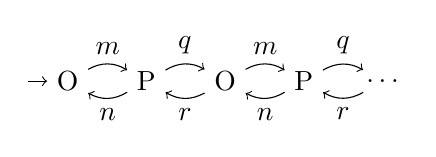
\begin{tikzpicture}[baseline=(O1.base)]
    \node (O1) at (0,0) {\kw{O}};
    \node (P1) at (1,0) {\kw{P}};
    \node (O2) at (2,0) {\kw{O}};
    \node (P2) at (3,0) {\kw{P}};
    \node (O3) at (4,0) {$\ldots$};
    \path [->] (-0.5,0) edge (O1);
    \path [->] (O1) edge[bend left] node[auto] {$m$} (P1);
    \path [->] (P1) edge[bend left] node[auto] {$n$} (O1);
    \path [->] (P1) edge[bend left] node[auto] {$q$} (O2);
    \path [->] (O2) edge[bend left] node[auto] {$r$} (P1);
    \path [->] (O2) edge[bend left] node[auto] {$m$} (P2);
    \path [->] (P2) edge[bend left] node[auto] {$n$} (O2);
    \path [->] (P2) edge[bend left] node[auto] {$q$} (O3);
    \path [->] (O3) edge[bend left] node[auto] {$r$} (P2);
  \end{tikzpicture}
  \quad
  \begin{array}{c@{\,}l@{\quad}c@{\,}l}
    m &\in M_B^\kw{Q} & q &\in M_A^\kw{Q} \\[1ex]
    n &\in M_B^\kw{A} & r &\in M_A^\kw{A}
  \end{array}
\]
The first move is always a question $m$ played by $\kw{O}$ in $B$.
The player $\kw{P}$ can conclude the current instance of $B$
with an answer $n$, or
initiate an instance of $A$
with a question $q$.
Then $\kw{O}$ can initiate a new instance of $B$
with another $m$, or
conclude any current instance of $A$
with an answer $r$.
This process goes on indefinitely.

%}}}

\subsubsection{Innocent strategies} %{{{

Readers familiar with traditional work on HON games \cite{something}
will recognize this description
as the \emph{well-bracketed} plays for the game ${!}A \multimap {!}B$
whose arena can be given schematically as:
\[
  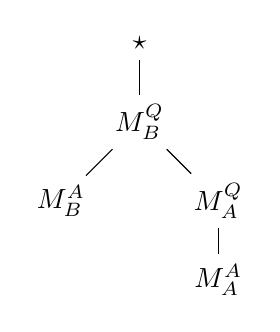
\begin{tikzpicture}
    \node (S) at (0,3) {$\star$};
    \node (BQ) at (0,2) {$M_B^\kw{Q}$};
    \node (BA) at (-1,1) {$M_B^\kw{A}$};
    \node (AQ) at (+1,1) {$M_A^\kw{Q}$};
    \node (AA) at (+1,0) {$M_A^\kw{A}$};
    \path (S) edge (BQ);
    \path (BQ) edge (BA);
    \path (BQ) edge (AQ);
    \path (AQ) edge (AA);
  \end{tikzpicture}
\]
Drawing from this work,
we can further distinguish \emph{innocent} strategies,
which handle all incoming questions $m \in M_B^\kw{Q}$
independently of the computation's history,
and therefore can be described in a particularly simple way.

Using elementary games as objects and innocent strategies as morphisms,
we can construct the following category.

\begin{definition}
The category $\mathcal{G}_i$
has the elementary games as objects,
and the interactive computations of the following type as morphisms:
\[
  \mathcal{G}_i(A, B) :=
  M_B^\kw{Q} \rightarrow \mathcal{I}_{M_A^\kw{Q},M_A^\kw{A}}(M_B^\kw{A}) \,.
\]
The identity morphism for $A$ is given by:
\[
  \kw{id}_A := \kw{interact}_{M_A^\kw{Q},M_A^\kw{A}} \,,
\]
and the composition of the morphisms
$f : A \rightarrow B$ and
$g : B \rightarrow C$
is given by:
\[
  g \circ f := m \mapsto g(m)[f] \,.
\]
[XXX actually define $x[f]$
in the interaction section,
and show relevant properties]
\end{definition}

%}}}

\subsubsection{Products} %{{{

As usual,
the product of elementary games $A \times B$




---

To formalize the plays and strategies of $A \rightarrow B$
in a way that accounts for refinement,
we decouple two aspects of this structure.
The following definition of plays
enforces the alternation between $\kw{O}$ and $\kw{P}$.

\begin{definition} % arrow game {{{
Given two elementary games $A$ and $B$,
the moves of the arrow game $A \rightarrow B$
are the questions and answers of $A$ and $B$,
categorized as follows:
\begin{align*}
  M_{A \rightarrow B}^\kw{O} &= M_A^\kw{A} + M_B^\kw{Q} &
  M_{A \rightarrow B}^\kw{Q} &= M_A^\kw{Q} + M_B^\kw{Q} \\
  M_{A \rightarrow B}^\kw{P} &= M_A^\kw{Q} + M_B^\kw{A} &
  M_{A \rightarrow B}^\kw{A} &= M_A^\kw{A} + M_B^\kw{A}
\end{align*}
The \emph{plays} are taken in
the prefix closure $P_{A \rightarrow B}$ of the set:
\[
    (M_{A \rightarrow B}^\kw{O}
     M_{A \rightarrow B}^\kw{P})^* \,
    (\varepsilon +
     M_{A \rightarrow B}^\kw{O} \Delta +
     M_{A \rightarrow B}^\kw{O} \lightning) \,.
\]
Note that
even-length plays represent positions where $\kw{O}$ is expected to play,
whereas odd-length plays represent positions where $\kw{P}$ is.
We write $P_{A \rightarrow B}^\kw{even}$ and $P_{A \rightarrow B}^\kw{odd}$
for the corresponding subsets of $P_{A \rightarrow B}$.
\end{definition}
%}}}

The ``stack discipline'' associating questions
with their eventual answer is captured by
the way we extend refinement conventions to
the plays of $A \rightarrow B$.

\begin{definition} % F_A->B %{{{
Given
$\mathbb{C}_A : \mathcal{R}(A_1, A_2)$ and
$\mathbb{C}_B : \mathcal{R}(B_1, B_2)$,
we can define the following relations
between the moves of $A_1 \rightarrow B_2$
and the moves of $A_2 \rightarrow B_2$:
\begin{align*}
  {\preceq}_{\mathbb{C}_A \rightarrow \mathbb{C}_B}^\kw{O} &=
    {\preceq}_{\mathbb{C}_A}^\kw{A} +
    {\preceq}_{\mathbb{C}_B}^\kw{Q} &
  {\preceq}_{\mathbb{C}_A \rightarrow \mathbb{C}_B}^\kw{Q} &=
    {\preceq}_{\mathbb{C}_A}^\kw{Q} +
    {\preceq}_{\mathbb{C}_B}^\kw{Q} \\
  {\preceq}_{\mathbb{C}_A \rightarrow \mathbb{C}_B}^\kw{P} &=
    {\preceq}_{\mathbb{C}_A}^\kw{Q} +
    {\preceq}_{\mathbb{C}_B}^\kw{A} &
  {\preceq}_{\mathbb{C}_A \rightarrow \mathbb{C}_B}^\kw{A} &=
    {\preceq}_{\mathbb{C}_A}^\kw{A} +
    {\preceq}_{\mathbb{C}_B}^\kw{A} \,,
\end{align*}
The Kripke frame
$\mathcal{F}_{\mathbb{C}_A \rightarrow \mathbb{C}_B} =
 \langle W_{\mathbb{C}_A \rightarrow \mathbb{C}_B}, \leadsto \rangle$
has worlds in
$W_{\mathbb{C}_A \rightarrow \mathbb{C}_B} =
 (W_{\mathbb{C}_A} + W_{\mathbb{C}_B})^*$,
and its accessibility relation $\leadsto$
relates moves of $A_1 \rightarrow B_1$
to moves of $A_2 \rightarrow B_2$,
as defined by the rules:
\[
    \AxiomC{$m_1 \ifr{w \Vdash {\preceq}_{\mathbb{C}_A \rightarrow \mathbb{C}_B}^\kw{Q}} m_2$}
    \UnaryInfC{$\vec{w} \stackrel{m_1, m_2}{\leadsto} w :: \vec{w}$}
    \DisplayProof
    \quad
    %\begin{array}{c}
    %  \vec{w} \stackrel{\#,\#}{\leadsto} \vec{w} \\[0.7ex]
    %  \vec{w} \stackrel{\tau, \tau}{\leadsto} \vec{w}
    %\end{array}
    %\quad
    \AxiomC{$m_1 \ifr{w \Vdash {\preceq}^\kw{A}_{\mathbb{C}_A \rightarrow \mathbb{C}_B}} m_2$}
    \UnaryInfC{$w :: \vec{w} \stackrel{m_1, m_2}{\leadsto} \vec{w} \,.$}
    \DisplayProof
\]
%Then two plays are related at $\vec{w}$
%when there is a path from $\varepsilon$ to $\vec{w}$
%in $\leadsto$ whose labels project onto the plays:
%\[
%    \AxiomC{$s : \varepsilon \leadsto^* \vec{w}$}
%    \UnaryInfC{$\pi_1^*(s)
%       \ifr{\vec{w} \Vdash {\preceq}_{A \rightarrow B}}
%       \pi_2^*(s)$}
%    \DisplayProof
%\]
%If
%$\langle A, \mathbb{C}_A \rangle$ and
%$\langle B, \mathbb{C}_B \rangle$
%are two games with refinement, then
%a \emph{valid play} of $A \rightarrow B$
%is a sequence $s \in P_{A \rightarrow B}$
%such that $(s, s) \in [\vec{w} \Vdash {\preceq}_{A \rightarrow B}]$
%for some $\vec{w}$.
\end{definition}

The frame $\mathcal{F}_{\mathbb{C}_A \rightarrow \mathbb{C}_B}$
is used in \S\ref{sec:sim}
to define our notion of simulation.
%}}}

%}}}

%}}}

\subsection{Strategies} %{{{

A strategy for $A \rightarrow B$
is essentially a tree
which gathers the possible interactions of
the system being modeled.
We give a traditional representation
as a prefix-closed set of plays,
but will work with strategies defined as transition systems.

\subsubsection{Traces} %{{{

In the existing literature,
strategies are usually formalized as prefix-closed sets of plays.
This establishes a connection with trace semantics of process calculi.
In our case,
a strategy given in this form is a set:
\[ \sigma \subseteq P_{A \rightarrow B} \,, \]
which satisfies
for all $st \in P_{A \rightarrow B}$
and $m \in M_{A \rightarrow B}^\kw{O}$:
\begin{itemize}
  \item $st \in \sigma \Rightarrow s \in \sigma$;
  \item $s\lightning \in \sigma \Rightarrow st \in \sigma$;
  \item $s \in \sigma \wedge sm \in P_{A \rightarrow B}
    \Rightarrow sm \in \sigma$.
\end{itemize}
The first condition ensures that $\sigma$ is prefix-closed.
It is complemented by the second condition,
which ensures that if a strategy goes wrong,
then it admits all other possible behaviors as well
from this point forward,
so that trace inclusion coincides with the notion of refinement
outlined in \S\ref{sec:bspec}.
The last condition ensures that
all possible behaviors of $\kw{O}$ are included
at all reachable positions.

%}}}

\subsubsection{Transition systems} %{{{

Instead of manipulating sets of traces directly,
we will define strategies using a specialized form of transition system.

\begin{definition} % strategy {{{
\label{def:strat}
An \emph{strategy} $\sigma$ for the arrow game $A \rightarrow B$
is a tuple
$\langle K, \delta, k_0 \rangle$
where:
\begin{itemize}
  \item $K$ is a set of \emph{continuation states};
  \item $\delta : K \rightarrow M_{A \rightarrow B}^\kw{O} \rightarrow
                  \mathcal{B}(M_{A \rightarrow B}^\kw{P} \times K)$
    specifies the behavior of each state
    for every possible opponent move;
  \item $k_0$
    is the strategy's \emph{initial continuation state}.
\end{itemize}
We write $\sigma : A \rightarrow B$ when $\sigma$ is a strategy
for $A \rightarrow B$.
\end{definition}
%}}}

Continuation states correspond to
the points in the execution where $\kw{O}$ is expected to move.
In reaction to an opponent move,
$\delta$ specifies which outcomes are possible:
the strategy may diverge, go wrong,
and specify successful outcomes
consisting of a proponent move,
together with a new continuation
which will be used to handle the next opponent move.

Accordingly,
the set of traces associated with a state is
defined recursively as:
\[
  \begin{array}{l@{\:}c@{\:\{}l@{\:\mid\:}l}
    \kw{traces}_\delta(k) & = & \varepsilon, m &
      m \in M_{A \rightarrow B}^\kw{O} \} \\
    & \cup & m \Delta &
      \delta(k, m) \ni \Delta \} \\
    & \cup & mt &
      \delta(k, m) \ni \lightning \wedge mt \in P_{A \rightarrow B} \} \\
    & \cup & m n t &
      \delta(k, m) \ni (n, k') \wedge t \in \kw{traces}_\delta(k') \}
  \end{array}
\]
Then the behavior of strategies can be made explicit
by specifying the corresponding sets of plays as:
\[
  \kw{traces}(\sigma) = \kw{traces}_\delta(k_0) \,.
\]

Formulated as transition systems,
the alternating structure of strategies
is ``baked into'' their definition.
This facilitates
mechanization in a proof assistant,
and facilitate a style of reasoning
which takes advantage of operational intuitions.

On the other hand,
in our approach strategies do not have a unique representation.
This is mitigated by the fact that
our primary concern will be refinement,
rather than equality of strategies:
we will mainly reason modulo simulations.

%}}}

%}}}

\subsection{Simulations} %{{{
\label{sec:sim}

Having formally defined a notion of strategy
for the game $A \rightarrow B$,
we turn to the corresponding relational notion of simulation
for the refinement convention $\mathbb{C}_A \rightarrow \mathbb{C}_B$.
To this end,
we first introduce the following modal constructions.

\begin{definition} % modal relators for simulation {{{
For frames labelled by pairs
($\Lambda = \Lambda_1 \times \Lambda_2$),
we define variants of $\Box, \Diamond$ which
allow world transitions to interact with the components
being related.
The relators:
\begin{align*}
  \Diamond \times {-} &: \mathcal{R}_W(A, B) \rightarrow
              \mathcal{R}_W(\Lambda_1 \times A, \, \Lambda_2 \times B) \\
  \Box \rightarrow - &: \mathcal{R}_W(A, B) \rightarrow
          \mathcal{R}_W(\Lambda_1 \rightarrow A, \, \Lambda_2 \rightarrow B)
\end{align*}
are defined as:
\begin{gather*}
  (l_1, a) \ifr{w \Vdash \Diamond \times R} (l_2, b) \Leftrightarrow
    a \ifr{w \Vdash \langle l_1, l_2 \rangle R} b \\
  f \ifr{w \Vdash \Box \rightarrow R} g \Leftrightarrow
    \forall \, l_1 l_2 \,.\, f(l_1) \ifr{w \Vdash [l_1, l_2] R} g(l_2)
\end{gather*}
\end{definition}
%}}}

With these constructions,
our notion of simulation relation
is naturally derived from
the type we used to define strategies (Def.~\ref{def:strat}).
They are used
with respect to the frame $\mathcal{F}_{A \rightarrow B}$
defined in \S\ref{sec:arrow}.
Hence, the simulation operates in the context of
a stack of elementary worlds
specifying how answers to pending questions
should be related.
In each one of the component games,
answers will be related at the same world as the corresponding questions:
$\kw{P}$ can rely on $\kw{O}$ making this true for the domain game;
it must guarantee that this is true for the codomain game.

\begin{definition} % simulation relation {{{
Given
$\mathbb{C}_A : \mathcal{R}(A_1, A_2)$,
$\mathbb{C}_B : \mathcal{R}(B_1, B_2)$
two refinement conventions, and
$\sigma_1 : A_1 \rightarrow B_1$,
$\sigma_2 : A_2 \rightarrow B_2$
two strategies,
a \emph{simulation relation} between $\sigma_1$ and $\sigma_2$
is a relation $R : \mathcal{R}_{W_{\!A \rightarrow B}}(K_1, K_2)$
such that:
\begin{gather*}
  \delta_1
  \ifr{\Vdash R \rightarrow \Box \rightarrow \mathcal{B}^+(\Diamond \times R)}
  \delta_2
  \\
  k_{0,1} \ifr{\varepsilon \Vdash R_K} k_{0,2}
\end{gather*}
We will write
$\sigma_1 \le_{\mathbb{C}_A \rightarrow \mathbb{C}_B}^R \sigma_2$
when $R$ is a simulation relation in this sense, and write
$\sigma_1 \le_{\mathbb{C}_A \rightarrow \mathbb{C}_B} \sigma_2$
when there exists any such simulation relation.
\end{definition}
%}}}

%}}}

\subsection{Constructions} %{{{

\subsubsection{Products} %{{{

The simplest way to aggregate a family of strategies $(\sigma_i)_{i \in I}$
is to annotate all of the moves by a component identifier $i$.
This corresponds to the categorical product.

\begin{definition} % Product game {{{
Given a family of elementary games $(A_i)_{i \in I}$,
we define their \emph{product} as the game:
\[ \prod_{i \in I} A_i =
   \Big\langle \sum_{i \in I} M_{A_i}^\kw{Q},
            \: \sum_{i \in I} M_{A_i}^\kw{A} \Big\rangle \,. \]
We will write $A_1 \times A_2 := \prod_{i \in \{1, 2\}} A_i$
and $A^I := \prod_{i \in I} A$.
\end{definition}
%}}}

The aggregated strategy uses the labels to direct each move
to the corresponding component,
and lets the components operate independently.

\begin{definition} % Product of strategies {{{
For a family of strategies
$(\sigma_i : A_i \rightarrow B_i)_{i \in I}$,
their product is the strategy
$\prod_i \sigma_i := \langle \prod_i K_i, \prod_i \delta_i, (k_i)_{i\in I} \rangle$,
where the relation
$\prod_i \delta_i$
is defined as:
\[
  (\vec{k}, (i, m)) \mapsto
    \delta_i(k_i, m) \bind (n, k_i') \mapsto ((i, n), \vec{k}[i := k_i']) \,.
\]
As before,
we write $\sigma_1 \times \sigma_2 := \prod_{i \in \{1, 2\}} \sigma_i$
and $\sigma^I := \prod_{i \in I} \sigma$.
\end{definition}
%}}}

%}}}

\subsubsection{Interaction} %{{{

While the product of two strategies
let them operate independently,
a construction like the composition $f \cdot g$ of
$f : A \rightarrow B$ and $g : B \rightarrow C$
is more subtle:
it involves the unbounded interaction of $f$ and $g$
over the common game $B$.

To model this interaction,
we introduce the following operator.
Given a strategy $\sigma : \Gamma \times A \rightarrow A \times \Delta$,
we will construct the strategy $Z(\sigma) : \Gamma \rightarrow \Delta$
by letting $\sigma$ interact with itself
over the game $A$ common to its domain and codomain.

\begin{definition}
Given $\sigma : \Gamma \times A \rightarrow A \times \Delta$,
we define the strategy $Z(\sigma) : \Gamma \rightarrow \Delta$
by iteration over the set of states:
\[
    S := K_\sigma \times (M_\Gamma + M_A + M_\Delta) \,.
\]
When a continuation of $Z(\sigma)$ is resumed by an opponent move,
we first store the move as a component of the state:
\begin{gather*}
  \kw{in} : K_\sigma \rightarrow
            M_{\Gamma \rightarrow \Delta}^\kw{O} \rightarrow
            \mathcal{B}(S) \\
  \kw{in}_k(m) := \{ (k, m) \}
\end{gather*}
Then, we will let $\sigma$ act on the state
by lifting its transition relation to $S$.
Given the obvious injections:
\begin{align*}
  \iota_\kw{O} &:
    M_{\Gamma \times A \rightarrow A \times \Delta}^\kw{O}
    \rightarrow
    M_\Gamma + M_A + M_\Delta \\
  \iota_\kw{P} &:
    M_{\Gamma \times A \rightarrow A \times \Delta}^\kw{P}
    \rightarrow
    M_\Gamma + M_A + M_\Delta \,,
\end{align*}
we define the relation
$\kw{step} : S \rightarrow \mathcal{B}(S)$
using the rule:
\[
  \kw{step}(k, \iota_\kw{O}(m)) =
    \delta_\sigma(k, m) \bind (m', k') \mapsto (k', \iota_\kw{P}(m')) \,,
\]
with the understanding that $\kw{step}(k, m) = \bot$
whenever the current move $m$ is
in $M_\Gamma^\kw{Q}$ or $M_\Delta^\kw{A}$.
When we reach such a move,
we instead return control to the environment:
\begin{gather*}
  \kw{out} : S \rightarrow
    \mathcal{B}(M_{\Gamma \rightarrow \Delta}^\kw{P} \times K) \\
  \kw{out}(k, m) =
    \{ (m, k) \mid m \in M_{A \rightarrow B}^\kw{P} \}
\end{gather*}
With these, the strategy $Z(\sigma)$ can be defined as:
\[
    Z(\sigma) := \langle
       K_\sigma, \:
       k \mapsto \kw{in}_k \cdot \kw{step}^* \cdot \kw{out}, \:
       k_{0\sigma}
     \rangle \,.
\]
\end{definition}

%}}}

\subsubsection{Identity and composition} %{{{

With products and the interaction combinator $Z$,
we can define the categorical composition of
$f : A \rightarrow B$ and $g : B \rightarrow C$ as:
\[
    f \cdot g := Z(f \times g) \,.
\]
The identity strategy $\kw{id}_A : A \rightarrow A$
simply passes codomain questions to the domain game,
and passes domain answers back to the codomain.
It is defined as:
$\kw{id}_A := \langle \{ * \}, \delta_\kw{id}, * \rangle$,
with $\delta_\kw{id}(*, m) = \{(m, *)\}$.

%}}}

\subsubsection{Duplication} %{{{

Although we have defined the product of strategies
$\prod_i \sigma_i : \prod_i A_i \rightarrow \prod_i B_i$,
we have not yet defined the tupling operation
$\langle \sigma_i \rangle_{i \in I}$
distinguishing the cartesian product
from weaker monoidal structures.
To this end,
we introduce the diagonal morphism
$\Delta_A^I : A \rightarrow A^I$.

The diagonal morphism simply passes through any
opponent question from a component $i \in I$ of its codomain
as a proponent question in its domain.
To make sure the answer can be routed back to $i$,
we remember which component of the codomain initiated
each pending question.
Hence,
the continuations of $\Delta$
consist of a stack $\iota \in I^*$
of component identifiers.

\begin{definition}[Diagonal morphism] % diagnoal morphism {{{
For an elementary game $A$ and a set $I$,
we define the strategy:
\[ \Delta_A^I := \langle I^*, \delta_\Delta, \varepsilon \rangle
  : A \rightarrow A^I \,. \]
Writing $m \in M_A^\kw{Q}$ and $n \in M_A^\kw{A}$,
the transition relation $\delta_\Delta$
is defined by the rules:
\begin{align*}
  \delta_\Delta(\iota, (i, m)) &\ni (m, i :: \iota) & m &\in M_A^\kw{Q} \\
  \delta_\Delta(i :: \iota, n) &\ni ((i, n), \iota) & n &\in M_A^\kw{A} \,.
\end{align*}
Then for a family of strategies $(\sigma_i : A \rightarrow B_i)_{i \in I}$,
we define
$\langle \sigma_i \rangle_{i \in I} : A \rightarrow \prod_i B_i$
as the strategy:
\[
    \langle \sigma_i \rangle_{i \in I} := 
      \Delta^I \cdot \prod_i \sigma_i \,.
\]
\end{definition}
%}}}

%}}}

\subsubsection{Choice} %{{{

Because our underlying notion of behavior supports
nondeterministic choice,
in addition to the diagonal morphism
$\Delta : A \rightarrow A^I$,
we can define a strategy
$\Sigma : A^I \rightarrow A$
which will pass each opponent question in the codomain
to a nondeterministically chosen component in the domain.

\begin{definition}
For an elementary game $A$ and a set $I$,
the strategy $\Sigma_A^I : A^I \rightarrow A$
is defined as $\langle \{*\}, \delta_\Sigma, * \rangle$
where $\delta_\Sigma$ is defined by the rules:
\begin{align*}
  &\delta_\Sigma(*, m) \ni \{((i, m), *)\} & m &\in M_A^\kw{Q} \\
  &\delta_\Sigma(*, (i, n)) \ni \{(n, *)\} & n &\in M_A^\kw{A} \,.
\end{align*}
For $f, g : A \rightarrow B$,
the strategy $f \oplus g$ is defined as:
\[ f \oplus g := \Delta \cdot (f \times g) \cdot \Sigma \,. \]
\end{definition}

This construction allows us to complement
the multiplicative structure $\langle \cdot, \kw{id} \rangle$
of our game model
with an additive component $\langle \oplus, \bot \rangle$.
The additive identity is defined as the empty strategy
$\bot_{A,B} := \langle \{*\}, * \mapsto 0, * \rangle : A \rightarrow B$.
The strategy $f \oplus g$
implements a form of continuous nondeterministic choice between $f$ and $g$:
for each incoming question in $M_B^\kw{Q}$,
the operator will nondeterministically route it to either $f$ or $g$.

%}}}

\subsubsection{Iterated composition}

The logical next step is to define the Kleene star
associated with $\cdot$ and $\oplus$.
Given a strategy $\sigma : A \rightarrow A$,
we define:
\begin{align*}
  \sigma^{\oplus} &:= Z(\Sigma \cdot \sigma \cdot \Delta) \\
  \sigma^{\oast} &:= \sigma^{\oplus} \oplus \kw{id}_A
\end{align*}

Once again,
the structure
$\langle \mathcal{G}[A,A], \cdot, \kw{id}, \oplus, \bot, {}^\oast \rangle$
does not define a Kleene algebra,
because $\bot$ may not act as an absorbing element
on the left of $\cdot$.
Nevertheless,
these operations will allow us to construct
more complex operators on strategies,
such as the horizontal composition of CompCert components
defined in \S\ref{sec:hcomp},
and to use equational reasoning to
establish properties of these operators.

%}}}

\subsection{Relational properties} %{{{

XXX: I want to show that all of the basic constructions
are compatible with simulations.
The junk below is outdated but contains
definitions of simulation relations that I should be able
to reuse.

{ \color{gray} %{{{

Furthermore,
for a refinement convention
$\mathbb{C} : \mathbb{R}_{W}(A_1, A_2)$,
the relation $R_\kw{id}$ defined by the single rule:
\[
    \AxiomC{$\vec{w} = w_1 w_1 \cdots w_n w_n$}
    \UnaryInfC{$* \ifr{\vec{w} \Vdash R_\kw{id}} *$}
    \DisplayProof
\]
is such that
$\kw{id}_{\!A_1} \le_{\mathbb{C} \rightarrow \mathbb{C}}^{R_\kw{id}} \kw{id}_{\!A_2}$.

\begin{definition}
For a family of refinement conventions
$(\mathbb{C}_i : \mathcal{R}(A_i, B_i))_{i \in I}$,
we define:
\[ \prod_{i \in I} \mathbb{C}_i =
   \langle W, {\preceq}^\kw{Q}, {\preceq}^\kw{A} \rangle :
   \mathcal{R}\Big(\prod_i A_i, \prod_i B_i \Big) \]
where
$W = \sum_i W_{\mathbb{C}_i}$ and
$\preceq^\kw{Q}, \preceq^\kw{A}$
are given by the rules:
\[
    \small
    \AxiomC{$m_1 \ifr{w \Vdash {\preceq}_{\mathbb{C}_i}^\kw{Q}} m_2$}
    \UnaryInfC{$(i, m_1) \ifr{(i, w) \Vdash {\preceq}^\kw{Q}} (i, m_2)$}
    \DisplayProof
    \quad
    \AxiomC{$m_1 \ifr{w \Vdash {\preceq}_{\mathbb{C}_i}^\kw{A}} m_2$}
    \UnaryInfC{$(i, m_1) \ifr{(i, w) \Vdash {\preceq}^\kw{A}} (i, m_2)$}
    \DisplayProof
\]
\end{definition}

\begin{lemma} % monotonicity {{{
For a family of simulation relations $\vec{R} = (R_i)_{i \in I}$ such that
$\sigma_{1,i} \le_{\mathbb{C}_A \rightarrow \mathbb{C}_B}^{R_i} \sigma_{2,i}$,
the relation $\mathcal{M}(\vec{R})$ defined by:
\begin{gather*}
  \AxiomC{$\forall i \,.\,
    k_{1,i} \ifr{\vec{w} \restriction i \Vdash R_{K,i}} k_{2,i}$}
  \UnaryInfC{$\vec{k_1} \ifr{\vec{w} \Vdash \mathcal{M}(\vec{R})_K} \vec{k_2}$}
  \DisplayProof
  \\[.5ex]
  \AxiomC{$s_1 \ifr{\vec{w} \restriction i \Vdash R_{S,i}} s_2$}
  \AxiomC{$\forall j \ne i \,.\,
    k_{1,j} \ifr{\vec{w} \restriction j \Vdash R_{S,j}} k_{2,j}$}
  \BinaryInfC{$(i, s_1, \vec{k}_1)
    \ifr{\vec{w} \Vdash \mathcal{M}(\vec{R})_S}
    (i, s_2, \vec{k}_2)$}
  \DisplayProof
\end{gather*}
is a simulation relation between the strategies:
\[
  \mathcal{M}(\vec{\sigma_1})
  \le_{\mathbb{C}_A^I \rightarrow \mathbb{C}_B^I}^{\mathcal{M}(\vec{R})}
  \mathcal{M}(\vec{\sigma_2}) \, .
\]
The stack of worlds $\vec{w} \restriction i$
is the sequence $w_1, w_2, \ldots, w_n$
such that $(i, w_1), (i, w_2), \ldots, (i, w_n)$
is the subsequence of $\vec{w}$ containing worlds
paired with $i$ indices.
\end{lemma}
%}}}

\subsubsection{Flat composition} %{{{

Once we have such an aggregate,
we can ``flatten'' the communication between
the system and the environment
back to the unannotated game $A \rightarrow B$.

\begin{definition} % flattening {{{
The \emph{flattening} of $\sigma : A^I \rightarrow B^I$
is the strategy $\sigma^\rhd : A \rightarrow B$
defined over the sets of states
$K := K_\sigma \times I^*$ and
$S := S_\sigma \times I^*$ by the following rules:
\[
  \begin{array}{c@{\quad}c}
    \AxiomC{$k \xrightarrow{(i, m)}_\sigma s$}
    \AxiomC{$\forall \, j \ne i \,.\, k \: \#_{\!\sigma} \: (j, m)$}
    \BinaryInfC{$(k, \iota) \xrightarrow{m} (s, \iota)$}
    \DisplayProof
    &
    \AxiomC{$s \xrightarrow{(i, n)}_\sigma k$}
    \UnaryInfC{$(s, \iota) \xrightarrow{n} (k, \iota)$}
    \DisplayProof
    \\[1.5em]
    \AxiomC{$s \xrightarrow{(i, q)}_\sigma k$}
    \UnaryInfC{$(s, \iota) \xrightarrow{q} (k, i :: \iota)$}
    \DisplayProof
    &
    \AxiomC{$k \xrightarrow{(i, r)}_\sigma s$}
    \UnaryInfC{$(k, i :: \iota) \xrightarrow{r} (s, \iota)$}
    \DisplayProof
    \\[1.5em]
    \AxiomC{$s \xrightarrow{\tau}_\sigma s'$}
    \UnaryInfC{$(s, \iota) \xrightarrow{\tau} (s', \iota)$}
    \DisplayProof
    &
    \AxiomC{$\forall \,i\,.\, k \: \#_{\!\sigma} \: (i, m)$}
    \UnaryInfC{$(k, \iota) \:\#\: m$}
    \DisplayProof
  \end{array}
\]
\end{definition}
%}}}

We direct an incoming question in $B$
to a component $i$ when all other components reject it.
If the component then asks a question in the game $A$,
we save its identifier on the stack $\iota$,
so that the corresponding answer can be directed back to $i$.

\begin{lemma}
Given a simulation relation
$\sigma_1 \le_{\mathbb{C}_A^I \rightarrow \mathbb{C}_B^I}^R \sigma_2$,
the relation $R^\rhd$ is defined for continuation states by:
\[
  \AxiomC{$k_1 \ifr{\vec{w} \Vdash R_K} k_2$}
  \AxiomC{$\iota = \pi_1^*(\vec{w}) \mbox{ XXX}$}
  \BinaryInfC{
    $(k_1, \iota) \ifr{\pi_2^*(\vec{w}) \Vdash R^\rhd_K} (k_2, \iota)$}
  \DisplayProof
\]
and similarly for running states.
$R^\rhd$ is a simulation relation:
\[
    \sigma_1^\rhd
    \le_{\mathbb{C}_A \rightarrow \mathbb{C}_B}^{R^\rhd}
    \sigma_2^\rhd \,.
\]
\end{lemma}

Putting together multi-component strategies and flattening,
the \emph{flat composition} operator
$\mathcal{F} : [A \rightarrow B] \rightarrow [A \rightarrow B]$
is:
\[
    \mathcal{F}(\vec{\sigma}) := \mathcal{M}(\vec{\sigma})^\rhd
\]
This allows us to bundle multiple components of the same type,
however note that so far they do not interact with each other
(only to decide who's going to handle what question).

%}}}

\subsubsection{Resolution operator} %{{{

To allow interaction within a composite system,
we define the following resolution operator,
which feeds back a strategy's own questions to itself
whenever possible.

\begin{definition} % resolution {{{
The \emph{resolution} of $\sigma : A \rightarrow A$,
written $\mathcal{R}(\sigma)$,
is defined over the sets of states
$K := K_\sigma \times \{\kw{O}, \kw{P}\}^*$ and
$S := S_\sigma \times \{\kw{O}, \kw{P}\}^*$
by the following rules:
\[
  \begin{array}{cc}
    {\small m \in M_A^\kw{Q}, \:\: n \in M_A^\kw{A}}
    &
    {\small q \in M_A^\kw{Q}, \:\: r \in M_A^\kw{A}}
    \\[1em]
    \AxiomC{$k \xrightarrow{m}_\sigma s$}
    \UnaryInfC{$(k, \iota) \xrightarrow{m} (s, \kw{O} :: \iota)$}
    \DisplayProof
    &
    \AxiomC{$s \xrightarrow{n}_\sigma k$}
    \UnaryInfC{$(s, \kw{O} :: \iota) \xrightarrow{n} (k, \iota)$}
    \DisplayProof
    \\[1.5em]
    \AxiomC{$s \xrightarrow{q}_\sigma k$}
    \AxiomC{$k \:\#_{\!\sigma}\: q$}
    \BinaryInfC{$(s, \iota) \xrightarrow{q} (k, \iota)$}
    \DisplayProof
    &
    \AxiomC{$k \xrightarrow{r}_\sigma s$}
    \UnaryInfC{$(k, \iota) \xrightarrow{r} (s, \iota)$}
    \DisplayProof
    \\[1.5em]
    \AxiomC{$s \xrightarrow{q}_\sigma k$}
    \AxiomC{$k \xrightarrow{q}_\sigma s'$}
    \BinaryInfC{$(s, \iota) \xrightarrow{\tau} (s', \kw{P} :: \iota)$}
    \DisplayProof
    &
    \AxiomC{$s \xrightarrow{r}_\sigma k$}
    \AxiomC{$k \xrightarrow{r}_\sigma s'$}
    \BinaryInfC{$(s, \kw{P} :: \iota) \xrightarrow{\tau} (s', \iota)$}
    \DisplayProof
    \\[1.5em]
    \AxiomC{$s \xrightarrow{\tau}_\sigma s'$}
    \UnaryInfC{$(s, \iota) \xrightarrow{\tau} (s', \iota)$}
    \DisplayProof
    &
    \AxiomC{$k \:\#_{\!\sigma}\: m$}
    \UnaryInfC{$(k, \iota) \:\#\: m$}
    \DisplayProof
  \end{array}
\]
The initial continuation is $(k_{\sigma}, \varepsilon)$.
\end{definition}
%}}}

\begin{lemma}
If
$\sigma_1 \le_{\mathbb{C}_A \rightarrow \mathbb{C}_A}^R \sigma_2$,
then
$\mathcal{R}(\sigma_1)
 \le_{\mathbb{C}_A \rightarrow \mathbb{C}_A}^{\mathcal{R}(R)}
 \mathcal{R}(\sigma_2)$,
where $\mathcal{R}(R)$ is defined as follows.
For a world $\vec{w} \in W_{A \rightarrow B}$
and a stack $\iota \in \{\kw{O}, \kw{P}\}^*$,
the set $\mathcal{R}_\iota(\vec{w}) \subseteq W_{A \rightarrow B}$
is defined by the following rules together with the base case
$\varepsilon \in \mathcal{R}_\varepsilon(\varepsilon)$:
\[
    \AxiomC{$\vec{w}' \in \mathcal{R}_\iota(\vec{w})$}
    \UnaryInfC{$x :: \vec{w}' \in \mathcal{R}_{\kw{O} :: \iota}(x :: \vec{w})$}
    \DisplayProof
    \quad
    \AxiomC{$\vec{w}' \in \mathcal{R}_\iota(\vec{w})$}
    \UnaryInfC{$x :: x :: \vec{w}' \in \mathcal{R}_{\kw{P} :: \iota}(\vec{w})$}
    \DisplayProof
\]
XXX this is only the rules for codomain worlds,
we need a case for domain worlds to be passed along.

Then the relation $\mathcal{R}(R)$ is given for continuation states by:
\[
  \AxiomC{$k_1 \ifr{\vec{w} \Vdash R_K} k_2$}
  \AxiomC{$\vec{w}' \in \mathcal{R}_\iota(\vec{w})$}
  \BinaryInfC{$(k_1, \iota) \ifr{\vec{w}' \Vdash \mathcal{R}(R)_K} (k_2, \iota)$}
  \DisplayProof
\]
and similarly for running states.

XXX the proof needs $\mathcal{R}(\vec{w})$ to take into account
whether the component is currently running (states) or not (continuations).
\end{lemma}

%}}}

\subsubsection{Observation operator} %{{{

The simulations defined in \S\ref{sec:sim}
only relate strategies whose internal actions match one-to-one.
However, the operator defined in this section
will allow us to normalize strategies by removing
all finite sequences of $\tau$s.

\begin{definition}
Given $\sigma : A \rightarrow B$,
the \emph{observation strategy}
$\sigma \backslash \tau^* =
 \langle K_\sigma, S_\sigma \uplus \{\ast\},
         \xrightarrow{\kw{O}},
         \xrightarrow{\tau},
         \xrightarrow{\kw{P}}_\sigma,
         \#_\sigma, k_{0,\sigma} \rangle$
uses the resumption and internal transition relations
defined by the rules:
\[
  \AxiomC{$s \xrightarrow{\tau}_\sigma s'$}
  \AxiomC{$s' \xrightarrow{\tau^\omega}$}
  \doubleLine \BinaryInfC{$s \xrightarrow{\tau^\omega}$}
  \DisplayProof
  \qquad
  \AxiomC{$k \xrightarrow{m}_\sigma s$}
  \AxiomC{$s \xrightarrow{\tau^\omega}$}
  \BinaryInfC{$k \xrightarrow{m} \ast$}
  \DisplayProof
\]\[
  \AxiomC{$k \xrightarrow{m}_\sigma s$}
  \AxiomC{$s \xrightarrow{\tau^*}_\sigma s' \xrightarrow{n}_\sigma k'$}
  \BinaryInfC{$k \xrightarrow{m} s'$}
  \DisplayProof
  \qquad
  \ast \xrightarrow{\tau} \ast \,.
\]
\end{definition}

\begin{lemma}
If $\sigma_1 \le_{\mathbb{C}_A \rightarrow \mathbb{C}_B}^R \sigma_2$,
then for $R \backslash \tau^* = R \cup \{(\ast, \ast)\}$
the following holds:
\[
  \sigma_1 \backslash \tau^*
  \le_{\mathbb{C}_A \rightarrow \mathbb{C}_B}^{R \backslash \tau^*}
  \sigma_2 \backslash \tau^* \,.
\]
\end{lemma}

%}}}

Note that for both states and continuations,
nondeterminism is interpreted as \emph{output} nondeterminism,
as prescribed by the use of the relator $\mathcal{P}^+$.
This means that alternating transition system
implicitely accept all possible inputs from the environment,
although some of them may cause the system to immediately go wrong.
Likewise,
the special resumption $\kw{refuse}$
is taken as a positive, output behavior from the system,
rather than a restriction on the environment ---
this will be important to establish the monotonicity
of the composition operator defined in Sec.~\ref{?}.
This approach corresponds to the saturation requirement on strategies
often found in traditional game semantics,
or notions of receptiveness used in CompCert
and in concurrency theory.

Furthermore, we need to distinguish between mere nondeterminism
and \emph{branching}.
This is explored in the following section.

\subsection{Branching and determinism}

Whereas nondeterminism allows a strategy to posess
multiple observable behaviors,
branching occurs when multiple state transitions
are associated with the same immediate observable behavior.
This can create spurious distinctions,
whereby systems that yield the same sets of traces
cannot be identified by simulation,
and as such we consider it undesirable.
The following definition
formalizes the conditions a transition system must satisfy
to be considered free from branching.

\begin{definition}[Nonbranching transition system]
For given sets of moves and states,
a continuation $k : M \rightarrow \mathcal{P}(\kw{resumption}(S))$
is \emph{nonbranching} if the following property holds:
\[ \forall m \,.\, | k(m) | \le 1 \]
A transition system $\alpha : \kw{ats}(M, S)$ is nonbranching
if the following property holds:
\[ \forall s, m, k_1, k_2 \,.\,
     \alpha(s) \supseteq \{ m \cdot k_1, m \cdot k_2 \} \Rightarrow
     k_1 = k_2 \,, \]
and if for all $s, m, k$ such that $\alpha(s) \ni \underline{m} \cdot k$,
the continuation $k$ is nonbranching.
\end{definition}

Determinism is a stronger property,
and ensures that the system has at most one possible behavior
at any point.
We expect the semantics of concrete systems ---
as opposed to specifications ---
to be deterministic in the following sense.

\begin{definition}[Deterministic transition system]
For given sets of moves and states,
a transition system $\alpha : \kw{ats}(M, S)$
is deterministic if for all $s$, $|\alpha(s)| \le 1$,
and if for all $s, m, k$ such that $\alpha(s) \ni \underline{m} \cdot k$,
the continuation $k$ is nonbranching.
\end{definition}

Note that both nonbranching and determinism
only relate to the behavior of the system.
In both cases,
the environment remains free to play any move.
Abramsky notes in \cite{cspgs}
that [it's one of the good things about game semantics].

\subsection{Internal actions and divergence}

The emergence of silent divergence
is one of the major difficulties
associated with modeling interacting systems.
Indeed,
two systems which, taken in isolation,
only exhibit reactive behavior,
can nonetheless become silently divergent when composed together,
if it is possible to interact with each other continuously
without intervening communication with the outside.

An operational description of this phenomenon
models this internal interaction explicitly
in the form of silent actions $\tau$.
When comparing the behavior of two systems,
finite sequences of $\tau$'s will be considered equivalent.
However,
silent divergence in the form of an infinite sequence of $\tau$'s
can only correspond to another infinite sequence.
This is usually addressed by the introduction of
sophisticated notions of simulation,
such as the \emph{measure simulations} used for instance in CompCert.

On the other hand,
in most work on denotational semantics,
including traditional game semantics such as \cite{pcfgs},
[complicated fixpoints] 

Our model includes a notion of internal action $\tau$,
which makes it possible to handle silent divergence explicitely
rather than through sophisticated domain-theoretic constructions.
However,
note that the notion of simulation we have defined
does not allow any variation
in the number of internal transitions
between the two transition systems being related.
Nevertheless,
composition operators remain monotonic
under this definition of simulation,
because [...]
Normalize using the following operator.

\begin{definition}[Observation operator]
For a transition system $\alpha : \kw{ats}(M, S)$,
we define the \emph{observations} transition system
$\mathcal{O}(\alpha)$ as follows.
A behavior $r : \kw{behavior}(M, S)$ is said to be
\emph{observable} if $r \ne \tau \cdot s$ for all $s \in S$.
A state $s' \in S$ is said to be \emph{reachable} from $s \in S$
if there is a sequence $s_0, s_1, \ldots s_n$ such that
$s_0 = s$, $s_n = s'$,
and for all $0 \le i < n$
there is a transition $\alpha(s_i) \ni \tau \cdot s_{i+1}$.
A state $s$ is said to be \emph{silently divergent}
if there is an infinite sequence $s_0, s_1, \ldots$
such that $s_0 = s$ and for all $i$,
there is a transition $\alpha(s_i) \ni \tau \cdot s_{i+1}$.
Then the observations transition system is defined as:
\begin{align*}
    \mathcal{O}(\alpha)(s) = &\{ r \:|\: r \mbox{ is observable } \wedge
         \exists s' \,.\, s \rightarrow^* s' \wedge
		\alpha(s') \ni r \} \\
      \cup &\{ \Delta \:|\: s \mbox{ is silently divergent} \}
\end{align*}
\end{definition}

Properties:
preserve nonbranching (if that's defined in the right way), determinism.
Monotonic.

}
%}}}
